\section{Implementation Considerations}

Since the core requirements of the project are architecture-independent to some degree, a simple solution which is not fully decentralised is a good option to begin with.

At current, a potential implementation utilises the following technologies:

\begin{outline}
  \1 AWS S3
  \1 AWS EB
  \1 AWS RDS
  \1 Ethereum
  \1 Electron
\end{outline}

The application would be distributed such that it could run on desktop operating systems (Mac and Linux (Debian) initially\footnote{Deployment of other packages may incur more overhead unnecessary at this point}). This means that the backend services of the project would be distinct from any front-end, whilst a public API offers the opportunity for third parties to contribute data and encourage user adoption.

The backend services of the project would be fulfilled to some extent by the following architecture:

\begin{figure}[H]
  \centering
  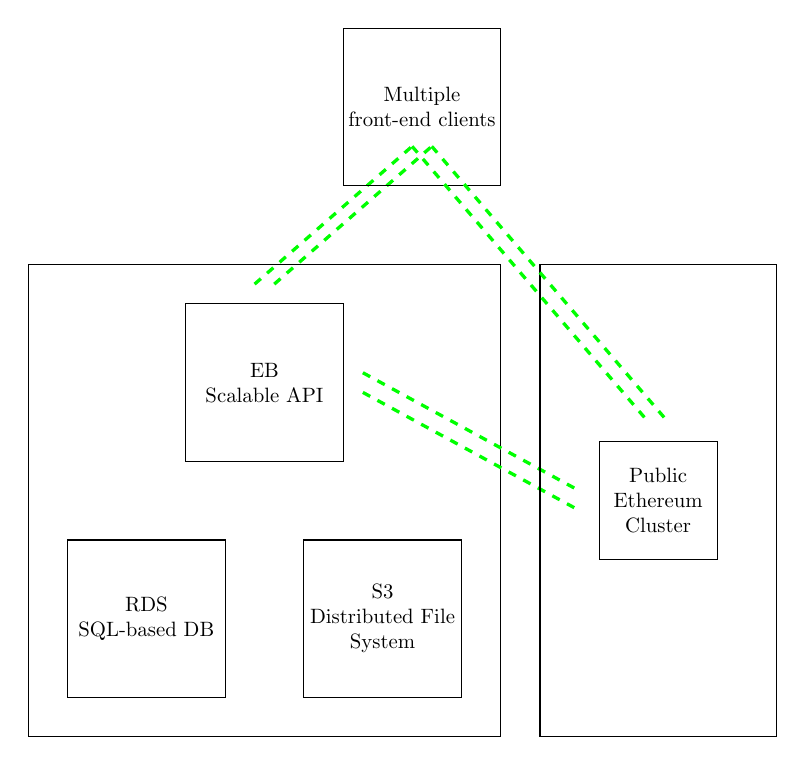
\begin{tikzpicture}[scale = 0.5, every node/.style={scale = 0.75}]

  % AWS Architecture
  \draw (-1, -1) rectangle (11, 11);
  \draw (0, 0) rectangle (4, 4);
  \draw (6, 0) rectangle (10, 4);
  \draw (3, 6) rectangle (7, 10);
  \draw[dashed, very thick, green] (4.75, 10.5) -- (8.75, 14);
  \draw[dashed, very thick, green] (5.25, 10.5) -- (9.25, 14);
  \draw[dashed, very thick, green] (7.5, 8.25) -- (13, 5.25);
  \draw[dashed, very thick, green] (7.5, 7.75) -- (13, 4.75);

  % Ethereum
  \draw (12, -1) rectangle (18, 11);
  \draw (13.5,  3.5) rectangle (16.5, 6.5);

  % Front-end services
  \draw (7, 13) rectangle (11, 17);
  \draw[dashed, very thick, green] (8.75, 14) -- (14.75, 7);
  \draw[dashed, very thick, green] (9.25, 14) -- (15.25, 7);

  \node[align=center] at (2, 2) { RDS\\SQL-based DB };
  \node[align=center] at (8, 2) { S3\\Distributed File\\System };
  \node[align=center] at (5, 8) { EB\\Scalable API };
  
  \node[align=center] at (9, 15) { Multiple\\front-end clients };
  
  \node[align=center] at (15, 5) { Public\\Ethereum\\Cluster };

  \end{tikzpicture}
  \caption{
    Potential architecture for proof of concept. Shows links between different systems using green, dashed lines. Each inner box referring to a specific service within a location (public or private). All links are made over public infrastructure.\textit{The Electron application that will be built as part of this proof of concept is assumed to be one of many front-end clients.}
  }
  \label{fig:arch_potential_1}
\end{figure}



